% Created by tikzDevice version 0.12.3.1 on 2023-04-20 20:50:44
% !TEX encoding = UTF-8 Unicode
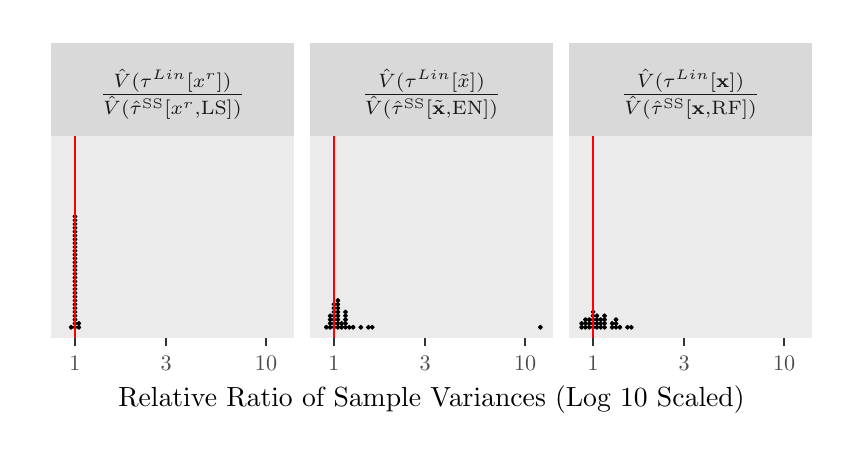
\begin{tikzpicture}[x=1pt,y=1pt]
\definecolor{fillColor}{RGB}{255,255,255}
\path[use as bounding box,fill=fillColor,fill opacity=0.00] (0,0) rectangle (289.08,144.54);
\begin{scope}
\path[clip] (  0.00,  0.00) rectangle (289.08,144.54);
\definecolor{drawColor}{RGB}{255,255,255}
\definecolor{fillColor}{RGB}{255,255,255}

\path[draw=drawColor,line width= 0.6pt,line join=round,line cap=round,fill=fillColor] (  0.00,  0.00) rectangle (289.08,144.54);
\end{scope}
\begin{scope}
\path[clip] (  8.25, 32.28) rectangle ( 96.36,105.24);
\definecolor{fillColor}{gray}{0.92}

\path[fill=fillColor] (  8.25, 32.28) rectangle ( 96.36,105.24);
\definecolor{drawColor}{RGB}{0,0,0}
\definecolor{fillColor}{RGB}{0,0,0}

\path[draw=drawColor,line width= 0.4pt,line join=round,fill=fillColor] ( 15.71, 36.28) circle (  0.69);

\path[draw=drawColor,line width= 0.4pt,line join=round,fill=fillColor] ( 17.09, 36.28) circle (  0.69);

\path[draw=drawColor,line width= 0.4pt,line join=round,fill=fillColor] ( 17.09, 37.66) circle (  0.69);

\path[draw=drawColor,line width= 0.4pt,line join=round,fill=fillColor] ( 17.09, 39.04) circle (  0.69);

\path[draw=drawColor,line width= 0.4pt,line join=round,fill=fillColor] ( 17.09, 40.43) circle (  0.69);

\path[draw=drawColor,line width= 0.4pt,line join=round,fill=fillColor] ( 17.09, 41.81) circle (  0.69);

\path[draw=drawColor,line width= 0.4pt,line join=round,fill=fillColor] ( 17.09, 43.19) circle (  0.69);

\path[draw=drawColor,line width= 0.4pt,line join=round,fill=fillColor] ( 17.09, 44.57) circle (  0.69);

\path[draw=drawColor,line width= 0.4pt,line join=round,fill=fillColor] ( 17.09, 45.95) circle (  0.69);

\path[draw=drawColor,line width= 0.4pt,line join=round,fill=fillColor] ( 17.09, 47.33) circle (  0.69);

\path[draw=drawColor,line width= 0.4pt,line join=round,fill=fillColor] ( 17.09, 48.71) circle (  0.69);

\path[draw=drawColor,line width= 0.4pt,line join=round,fill=fillColor] ( 17.09, 50.09) circle (  0.69);

\path[draw=drawColor,line width= 0.4pt,line join=round,fill=fillColor] ( 17.09, 51.47) circle (  0.69);

\path[draw=drawColor,line width= 0.4pt,line join=round,fill=fillColor] ( 17.09, 52.85) circle (  0.69);

\path[draw=drawColor,line width= 0.4pt,line join=round,fill=fillColor] ( 17.09, 54.24) circle (  0.69);

\path[draw=drawColor,line width= 0.4pt,line join=round,fill=fillColor] ( 17.09, 55.62) circle (  0.69);

\path[draw=drawColor,line width= 0.4pt,line join=round,fill=fillColor] ( 17.09, 57.00) circle (  0.69);

\path[draw=drawColor,line width= 0.4pt,line join=round,fill=fillColor] ( 17.09, 58.38) circle (  0.69);

\path[draw=drawColor,line width= 0.4pt,line join=round,fill=fillColor] ( 17.09, 59.76) circle (  0.69);

\path[draw=drawColor,line width= 0.4pt,line join=round,fill=fillColor] ( 17.09, 61.14) circle (  0.69);

\path[draw=drawColor,line width= 0.4pt,line join=round,fill=fillColor] ( 17.09, 62.52) circle (  0.69);

\path[draw=drawColor,line width= 0.4pt,line join=round,fill=fillColor] ( 17.09, 63.90) circle (  0.69);

\path[draw=drawColor,line width= 0.4pt,line join=round,fill=fillColor] ( 17.09, 65.28) circle (  0.69);

\path[draw=drawColor,line width= 0.4pt,line join=round,fill=fillColor] ( 17.09, 66.67) circle (  0.69);

\path[draw=drawColor,line width= 0.4pt,line join=round,fill=fillColor] ( 17.09, 68.05) circle (  0.69);

\path[draw=drawColor,line width= 0.4pt,line join=round,fill=fillColor] ( 17.09, 69.43) circle (  0.69);

\path[draw=drawColor,line width= 0.4pt,line join=round,fill=fillColor] ( 17.09, 70.81) circle (  0.69);

\path[draw=drawColor,line width= 0.4pt,line join=round,fill=fillColor] ( 17.09, 72.19) circle (  0.69);

\path[draw=drawColor,line width= 0.4pt,line join=round,fill=fillColor] ( 17.09, 73.57) circle (  0.69);

\path[draw=drawColor,line width= 0.4pt,line join=round,fill=fillColor] ( 17.09, 74.95) circle (  0.69);

\path[draw=drawColor,line width= 0.4pt,line join=round,fill=fillColor] ( 17.09, 76.33) circle (  0.69);

\path[draw=drawColor,line width= 0.4pt,line join=round,fill=fillColor] ( 18.47, 36.28) circle (  0.69);

\path[draw=drawColor,line width= 0.4pt,line join=round,fill=fillColor] ( 18.47, 37.66) circle (  0.69);
\definecolor{drawColor}{RGB}{255,0,0}

\path[draw=drawColor,line width= 0.6pt,line join=round] ( 17.09, 32.28) -- ( 17.09,105.24);
\end{scope}
\begin{scope}
\path[clip] (101.86, 32.28) rectangle (189.97,105.24);
\definecolor{fillColor}{gray}{0.92}

\path[fill=fillColor] (101.86, 32.28) rectangle (189.97,105.24);
\definecolor{drawColor}{RGB}{0,0,0}
\definecolor{fillColor}{RGB}{0,0,0}

\path[draw=drawColor,line width= 0.4pt,line join=round,fill=fillColor] (107.94, 36.28) circle (  0.69);

\path[draw=drawColor,line width= 0.4pt,line join=round,fill=fillColor] (109.32, 36.28) circle (  0.69);

\path[draw=drawColor,line width= 0.4pt,line join=round,fill=fillColor] (109.32, 37.66) circle (  0.69);

\path[draw=drawColor,line width= 0.4pt,line join=round,fill=fillColor] (109.32, 39.04) circle (  0.69);

\path[draw=drawColor,line width= 0.4pt,line join=round,fill=fillColor] (109.32, 40.43) circle (  0.69);

\path[draw=drawColor,line width= 0.4pt,line join=round,fill=fillColor] (110.70, 36.28) circle (  0.69);

\path[draw=drawColor,line width= 0.4pt,line join=round,fill=fillColor] (110.70, 37.66) circle (  0.69);

\path[draw=drawColor,line width= 0.4pt,line join=round,fill=fillColor] (110.70, 39.04) circle (  0.69);

\path[draw=drawColor,line width= 0.4pt,line join=round,fill=fillColor] (110.70, 40.43) circle (  0.69);

\path[draw=drawColor,line width= 0.4pt,line join=round,fill=fillColor] (110.70, 41.81) circle (  0.69);

\path[draw=drawColor,line width= 0.4pt,line join=round,fill=fillColor] (110.70, 43.19) circle (  0.69);

\path[draw=drawColor,line width= 0.4pt,line join=round,fill=fillColor] (110.70, 44.57) circle (  0.69);

\path[draw=drawColor,line width= 0.4pt,line join=round,fill=fillColor] (112.08, 36.28) circle (  0.69);

\path[draw=drawColor,line width= 0.4pt,line join=round,fill=fillColor] (112.08, 37.66) circle (  0.69);

\path[draw=drawColor,line width= 0.4pt,line join=round,fill=fillColor] (112.08, 39.04) circle (  0.69);

\path[draw=drawColor,line width= 0.4pt,line join=round,fill=fillColor] (112.08, 40.43) circle (  0.69);

\path[draw=drawColor,line width= 0.4pt,line join=round,fill=fillColor] (112.08, 41.81) circle (  0.69);

\path[draw=drawColor,line width= 0.4pt,line join=round,fill=fillColor] (112.08, 43.19) circle (  0.69);

\path[draw=drawColor,line width= 0.4pt,line join=round,fill=fillColor] (112.08, 44.57) circle (  0.69);

\path[draw=drawColor,line width= 0.4pt,line join=round,fill=fillColor] (112.08, 45.95) circle (  0.69);

\path[draw=drawColor,line width= 0.4pt,line join=round,fill=fillColor] (113.46, 36.28) circle (  0.69);

\path[draw=drawColor,line width= 0.4pt,line join=round,fill=fillColor] (113.46, 37.66) circle (  0.69);

\path[draw=drawColor,line width= 0.4pt,line join=round,fill=fillColor] (114.84, 36.28) circle (  0.69);

\path[draw=drawColor,line width= 0.4pt,line join=round,fill=fillColor] (114.84, 37.66) circle (  0.69);

\path[draw=drawColor,line width= 0.4pt,line join=round,fill=fillColor] (114.84, 39.04) circle (  0.69);

\path[draw=drawColor,line width= 0.4pt,line join=round,fill=fillColor] (114.84, 40.43) circle (  0.69);

\path[draw=drawColor,line width= 0.4pt,line join=round,fill=fillColor] (114.84, 41.81) circle (  0.69);

\path[draw=drawColor,line width= 0.4pt,line join=round,fill=fillColor] (116.22, 36.28) circle (  0.69);

\path[draw=drawColor,line width= 0.4pt,line join=round,fill=fillColor] (117.60, 36.28) circle (  0.69);

\path[draw=drawColor,line width= 0.4pt,line join=round,fill=fillColor] (120.37, 36.28) circle (  0.69);

\path[draw=drawColor,line width= 0.4pt,line join=round,fill=fillColor] (123.13, 36.28) circle (  0.69);

\path[draw=drawColor,line width= 0.4pt,line join=round,fill=fillColor] (124.51, 36.28) circle (  0.69);

\path[draw=drawColor,line width= 0.4pt,line join=round,fill=fillColor] (185.27, 36.28) circle (  0.69);
\definecolor{drawColor}{RGB}{255,0,0}

\path[draw=drawColor,line width= 0.6pt,line join=round] (110.70, 32.28) -- (110.70,105.24);
\end{scope}
\begin{scope}
\path[clip] (195.47, 32.28) rectangle (283.58,105.24);
\definecolor{fillColor}{gray}{0.92}

\path[fill=fillColor] (195.47, 32.28) rectangle (283.58,105.24);
\definecolor{drawColor}{RGB}{0,0,0}
\definecolor{fillColor}{RGB}{0,0,0}

\path[draw=drawColor,line width= 0.4pt,line join=round,fill=fillColor] (200.17, 36.28) circle (  0.69);

\path[draw=drawColor,line width= 0.4pt,line join=round,fill=fillColor] (200.17, 37.66) circle (  0.69);

\path[draw=drawColor,line width= 0.4pt,line join=round,fill=fillColor] (201.55, 36.28) circle (  0.69);

\path[draw=drawColor,line width= 0.4pt,line join=round,fill=fillColor] (201.55, 37.66) circle (  0.69);

\path[draw=drawColor,line width= 0.4pt,line join=round,fill=fillColor] (201.55, 39.04) circle (  0.69);

\path[draw=drawColor,line width= 0.4pt,line join=round,fill=fillColor] (202.93, 36.28) circle (  0.69);

\path[draw=drawColor,line width= 0.4pt,line join=round,fill=fillColor] (202.93, 37.66) circle (  0.69);

\path[draw=drawColor,line width= 0.4pt,line join=round,fill=fillColor] (202.93, 39.04) circle (  0.69);

\path[draw=drawColor,line width= 0.4pt,line join=round,fill=fillColor] (204.31, 36.28) circle (  0.69);

\path[draw=drawColor,line width= 0.4pt,line join=round,fill=fillColor] (204.31, 37.66) circle (  0.69);

\path[draw=drawColor,line width= 0.4pt,line join=round,fill=fillColor] (204.31, 39.04) circle (  0.69);

\path[draw=drawColor,line width= 0.4pt,line join=round,fill=fillColor] (204.31, 40.43) circle (  0.69);

\path[draw=drawColor,line width= 0.4pt,line join=round,fill=fillColor] (204.31, 41.81) circle (  0.69);

\path[draw=drawColor,line width= 0.4pt,line join=round,fill=fillColor] (205.69, 36.28) circle (  0.69);

\path[draw=drawColor,line width= 0.4pt,line join=round,fill=fillColor] (205.69, 37.66) circle (  0.69);

\path[draw=drawColor,line width= 0.4pt,line join=round,fill=fillColor] (205.69, 39.04) circle (  0.69);

\path[draw=drawColor,line width= 0.4pt,line join=round,fill=fillColor] (205.69, 40.43) circle (  0.69);

\path[draw=drawColor,line width= 0.4pt,line join=round,fill=fillColor] (207.07, 36.28) circle (  0.69);

\path[draw=drawColor,line width= 0.4pt,line join=round,fill=fillColor] (207.07, 37.66) circle (  0.69);

\path[draw=drawColor,line width= 0.4pt,line join=round,fill=fillColor] (207.07, 39.04) circle (  0.69);

\path[draw=drawColor,line width= 0.4pt,line join=round,fill=fillColor] (208.45, 36.28) circle (  0.69);

\path[draw=drawColor,line width= 0.4pt,line join=round,fill=fillColor] (208.45, 37.66) circle (  0.69);

\path[draw=drawColor,line width= 0.4pt,line join=round,fill=fillColor] (208.45, 39.04) circle (  0.69);

\path[draw=drawColor,line width= 0.4pt,line join=round,fill=fillColor] (208.45, 40.43) circle (  0.69);

\path[draw=drawColor,line width= 0.4pt,line join=round,fill=fillColor] (211.21, 36.28) circle (  0.69);

\path[draw=drawColor,line width= 0.4pt,line join=round,fill=fillColor] (211.21, 37.66) circle (  0.69);

\path[draw=drawColor,line width= 0.4pt,line join=round,fill=fillColor] (212.59, 36.28) circle (  0.69);

\path[draw=drawColor,line width= 0.4pt,line join=round,fill=fillColor] (212.59, 37.66) circle (  0.69);

\path[draw=drawColor,line width= 0.4pt,line join=round,fill=fillColor] (212.59, 39.04) circle (  0.69);

\path[draw=drawColor,line width= 0.4pt,line join=round,fill=fillColor] (213.98, 36.28) circle (  0.69);

\path[draw=drawColor,line width= 0.4pt,line join=round,fill=fillColor] (216.74, 36.28) circle (  0.69);

\path[draw=drawColor,line width= 0.4pt,line join=round,fill=fillColor] (218.12, 36.28) circle (  0.69);
\definecolor{drawColor}{RGB}{255,0,0}

\path[draw=drawColor,line width= 0.6pt,line join=round] (204.31, 32.28) -- (204.31,105.24);
\end{scope}
\begin{scope}
\path[clip] (  8.25,105.24) rectangle ( 96.36,139.04);
\definecolor{fillColor}{gray}{0.85}

\path[fill=fillColor] (  8.25,105.24) rectangle ( 96.36,139.04);
\definecolor{drawColor}{gray}{0.10}

\node[text=drawColor,anchor=base,inner sep=0pt, outer sep=0pt, scale=  1.00] at ( 52.31,125.21) {};

\node[text=drawColor,anchor=base,inner sep=0pt, outer sep=0pt, scale=  1.00] at ( 52.31,118.01) {$\frac{\hat{\mathbb{V}}(\tau^{Lin}[x^r])}{\hat{\mathbb{V}}(\hat{\tau}^{\mathrm{SS}}[x^r,\mathrm{LS}])}$};

\node[text=drawColor,anchor=base,inner sep=0pt, outer sep=0pt, scale=  1.00] at ( 52.31,110.81) {};
\end{scope}
\begin{scope}
\path[clip] (101.86,105.24) rectangle (189.97,139.04);
\definecolor{fillColor}{gray}{0.85}

\path[fill=fillColor] (101.86,105.24) rectangle (189.97,139.04);
\definecolor{drawColor}{gray}{0.10}

\node[text=drawColor,anchor=base,inner sep=0pt, outer sep=0pt, scale=  1.00] at (145.92,125.21) {};

\node[text=drawColor,anchor=base,inner sep=0pt, outer sep=0pt, scale=  1.00] at (145.92,118.01) {$\frac{\hat{\mathbb{V}}(\tau^{Lin}[\tilde{x}])}{\hat{\mathbb{V}}(\hat{\tau}^{\mathrm{SS}}[\tilde{\mathbf{x}},\mathrm{EN}])}$};

\node[text=drawColor,anchor=base,inner sep=0pt, outer sep=0pt, scale=  1.00] at (145.92,110.81) {};
\end{scope}
\begin{scope}
\path[clip] (195.47,105.24) rectangle (283.58,139.04);
\definecolor{fillColor}{gray}{0.85}

\path[fill=fillColor] (195.47,105.24) rectangle (283.58,139.04);
\definecolor{drawColor}{gray}{0.10}

\node[text=drawColor,anchor=base,inner sep=0pt, outer sep=0pt, scale=  1.00] at (239.52,125.21) {};

\node[text=drawColor,anchor=base,inner sep=0pt, outer sep=0pt, scale=  1.00] at (239.52,118.01) {$\frac{\hat{\mathbb{V}}(\tau^{Lin}[\mathbf{x}])}{\hat{\mathbb{V}}(\hat{\tau}^{\mathrm{SS}}[\mathbf{x},\mathrm{RF}])}$};

\node[text=drawColor,anchor=base,inner sep=0pt, outer sep=0pt, scale=  1.00] at (239.52,110.81) {};
\end{scope}
\begin{scope}
\path[clip] (  0.00,  0.00) rectangle (289.08,144.54);
\definecolor{drawColor}{gray}{0.20}

\path[draw=drawColor,line width= 0.6pt,line join=round] ( 17.09, 29.53) --
	( 17.09, 32.28);

\path[draw=drawColor,line width= 0.6pt,line join=round] ( 50.03, 29.53) --
	( 50.03, 32.28);

\path[draw=drawColor,line width= 0.6pt,line join=round] ( 86.14, 29.53) --
	( 86.14, 32.28);
\end{scope}
\begin{scope}
\path[clip] (  0.00,  0.00) rectangle (289.08,144.54);
\definecolor{drawColor}{gray}{0.30}

\node[text=drawColor,anchor=base,inner sep=0pt, outer sep=0pt, scale=  0.80] at ( 17.09, 20.71) {1};

\node[text=drawColor,anchor=base,inner sep=0pt, outer sep=0pt, scale=  0.80] at ( 50.03, 20.71) {3};

\node[text=drawColor,anchor=base,inner sep=0pt, outer sep=0pt, scale=  0.80] at ( 86.14, 20.71) {10};
\end{scope}
\begin{scope}
\path[clip] (  0.00,  0.00) rectangle (289.08,144.54);
\definecolor{drawColor}{gray}{0.20}

\path[draw=drawColor,line width= 0.6pt,line join=round] (110.70, 29.53) --
	(110.70, 32.28);

\path[draw=drawColor,line width= 0.6pt,line join=round] (143.64, 29.53) --
	(143.64, 32.28);

\path[draw=drawColor,line width= 0.6pt,line join=round] (179.75, 29.53) --
	(179.75, 32.28);
\end{scope}
\begin{scope}
\path[clip] (  0.00,  0.00) rectangle (289.08,144.54);
\definecolor{drawColor}{gray}{0.30}

\node[text=drawColor,anchor=base,inner sep=0pt, outer sep=0pt, scale=  0.80] at (110.70, 20.71) {1};

\node[text=drawColor,anchor=base,inner sep=0pt, outer sep=0pt, scale=  0.80] at (143.64, 20.71) {3};

\node[text=drawColor,anchor=base,inner sep=0pt, outer sep=0pt, scale=  0.80] at (179.75, 20.71) {10};
\end{scope}
\begin{scope}
\path[clip] (  0.00,  0.00) rectangle (289.08,144.54);
\definecolor{drawColor}{gray}{0.20}

\path[draw=drawColor,line width= 0.6pt,line join=round] (204.31, 29.53) --
	(204.31, 32.28);

\path[draw=drawColor,line width= 0.6pt,line join=round] (237.25, 29.53) --
	(237.25, 32.28);

\path[draw=drawColor,line width= 0.6pt,line join=round] (273.36, 29.53) --
	(273.36, 32.28);
\end{scope}
\begin{scope}
\path[clip] (  0.00,  0.00) rectangle (289.08,144.54);
\definecolor{drawColor}{gray}{0.30}

\node[text=drawColor,anchor=base,inner sep=0pt, outer sep=0pt, scale=  0.80] at (204.31, 20.71) {1};

\node[text=drawColor,anchor=base,inner sep=0pt, outer sep=0pt, scale=  0.80] at (237.25, 20.71) {3};

\node[text=drawColor,anchor=base,inner sep=0pt, outer sep=0pt, scale=  0.80] at (273.36, 20.71) {10};
\end{scope}
\begin{scope}
\path[clip] (  0.00,  0.00) rectangle (289.08,144.54);
\definecolor{drawColor}{RGB}{0,0,0}

\node[text=drawColor,anchor=base,inner sep=0pt, outer sep=0pt, scale=  1.00] at (145.91,  7.83) {Relative Ratio of Sample Variances (Log 10 Scaled)};
\end{scope}
\end{tikzpicture}
